\section{LSRs and \textit{MPLS clusters}}\label{cluster}
% %%%%%%%%%%%%%%%%%%%%%%%%%%%%%%%%%%%%%%
      
\begin{figure}[!t]
	\centering
		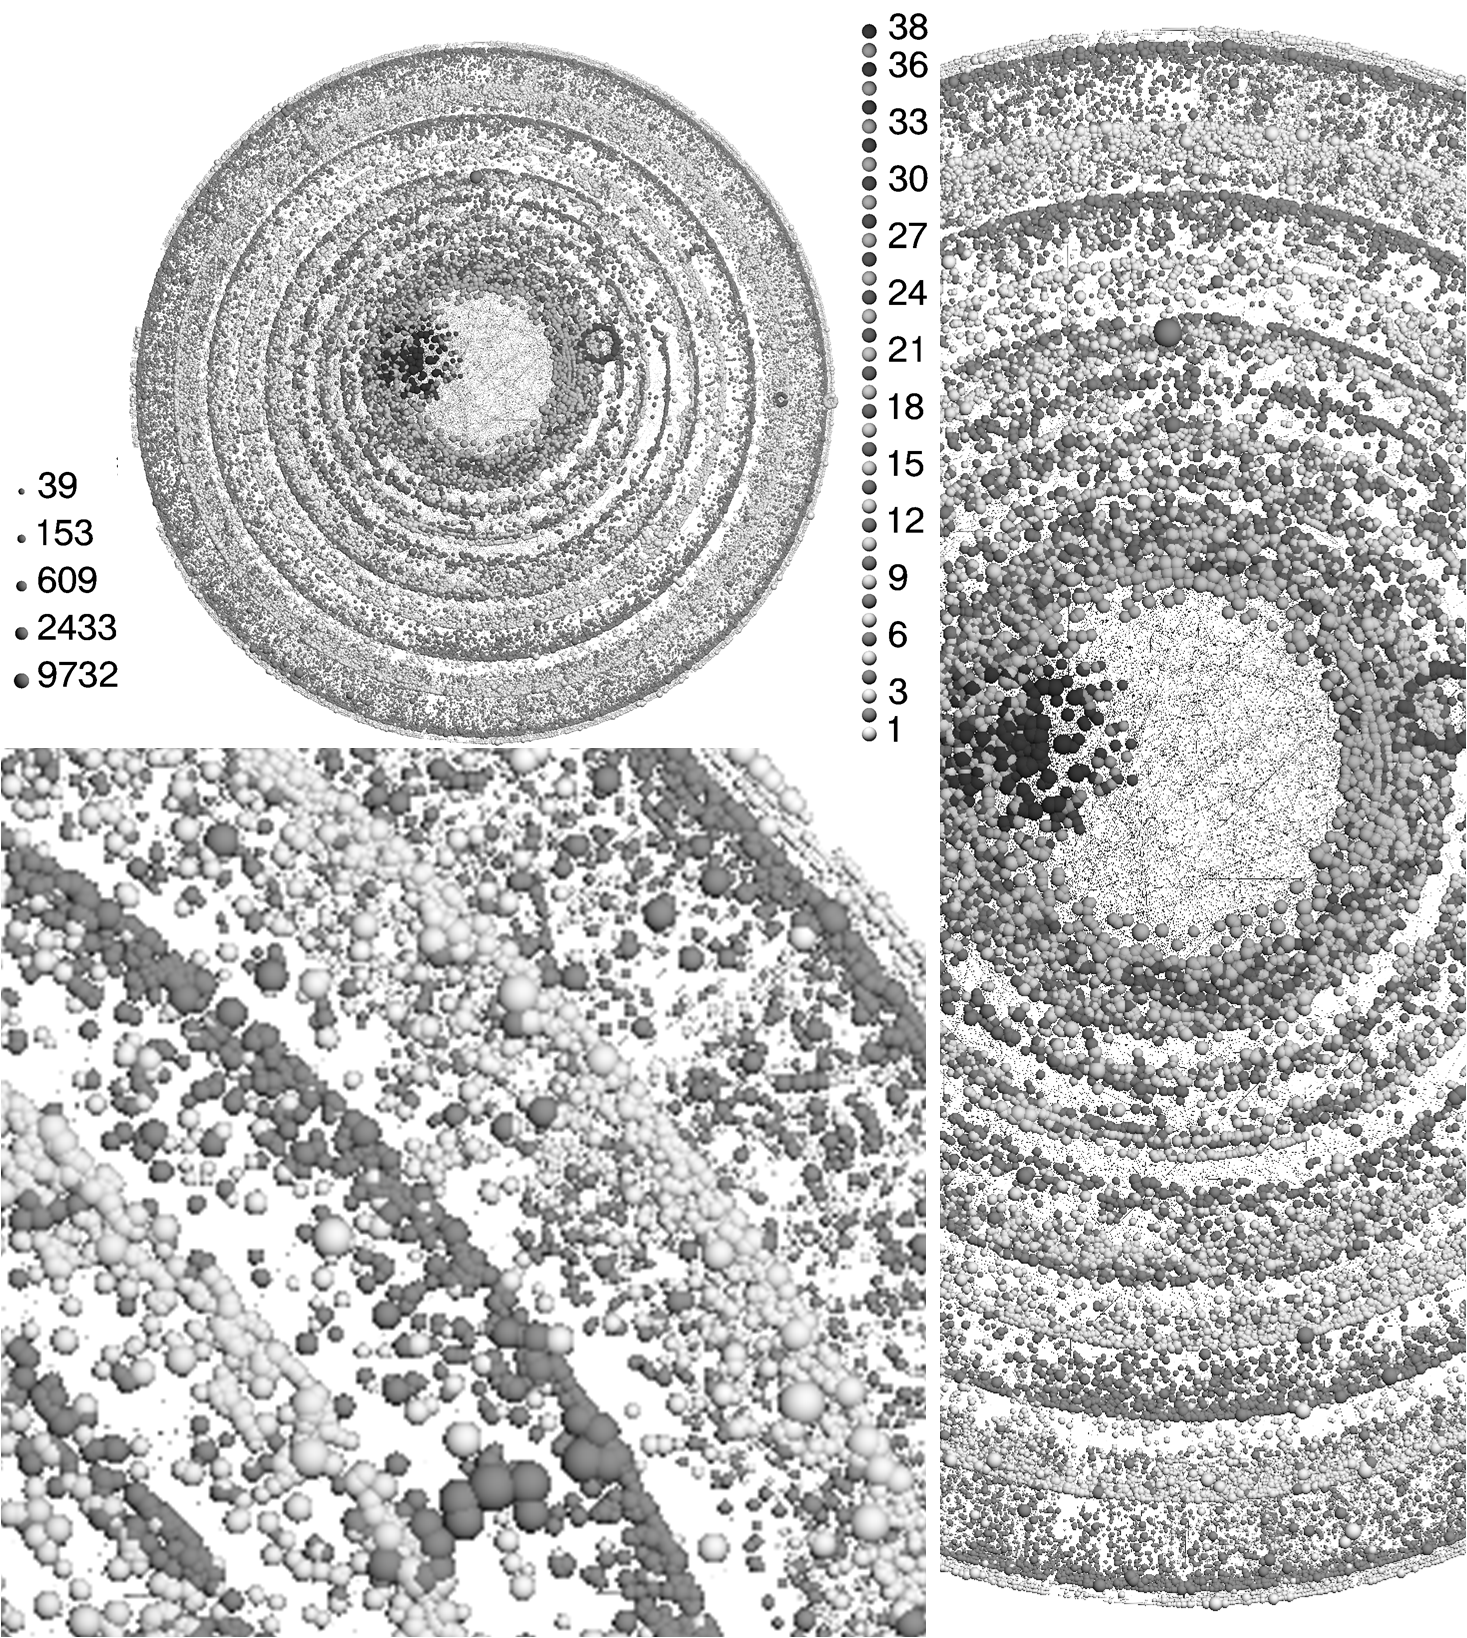
\includegraphics[width=3in]{Routers}
		\caption{$k$-core visualization of router level topology $G_{r}$ }
		\label{fig_k_core_routers}
\end{figure}

For the best of our acknowledge, MPLS interconnection architecture on Internet Topology has not been yet studied. 
In this way, in this section we focus our attention on study some properties of LSRs and \textit{MPLS clusters}; and their interaction with non MPLS networks. 
Our study aims to better understand the impact of MPLS deployments over internet, specifically over router level topology.

\subsection{Methodolody}\label{cluster.methodo}
% %%%%%%%%%%%%%%%%%%%%%%%

\begin{figure*}[!htb]
  \begin{center}
    \subfloat[Degree Distribution Probability]{\label{fig_degree_distribution}
      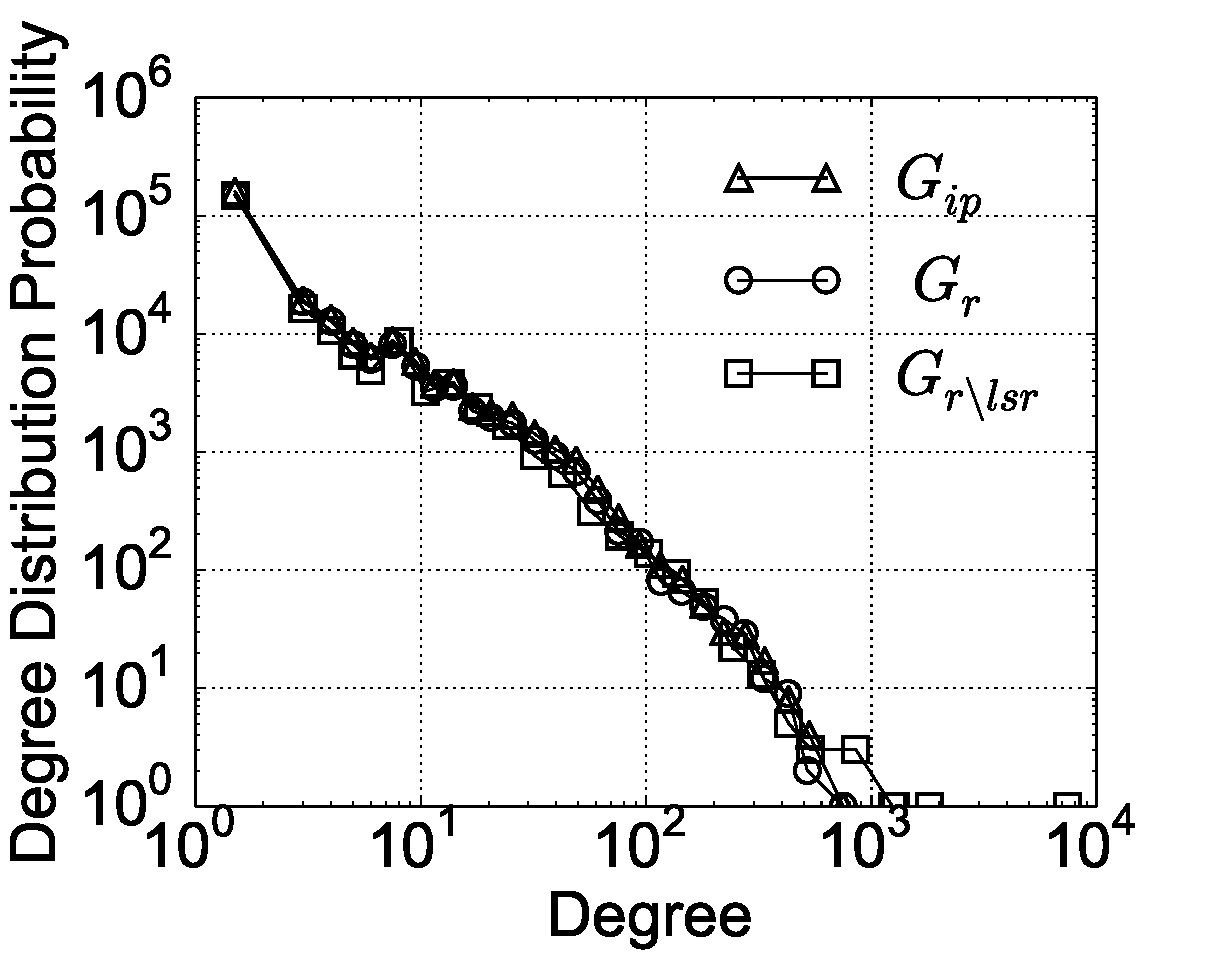
\includegraphics[width=5.5cm]{DegreeDistribution}}\hfil
    \subfloat[Clustering Coefficient]{\label{fig_clustering}
      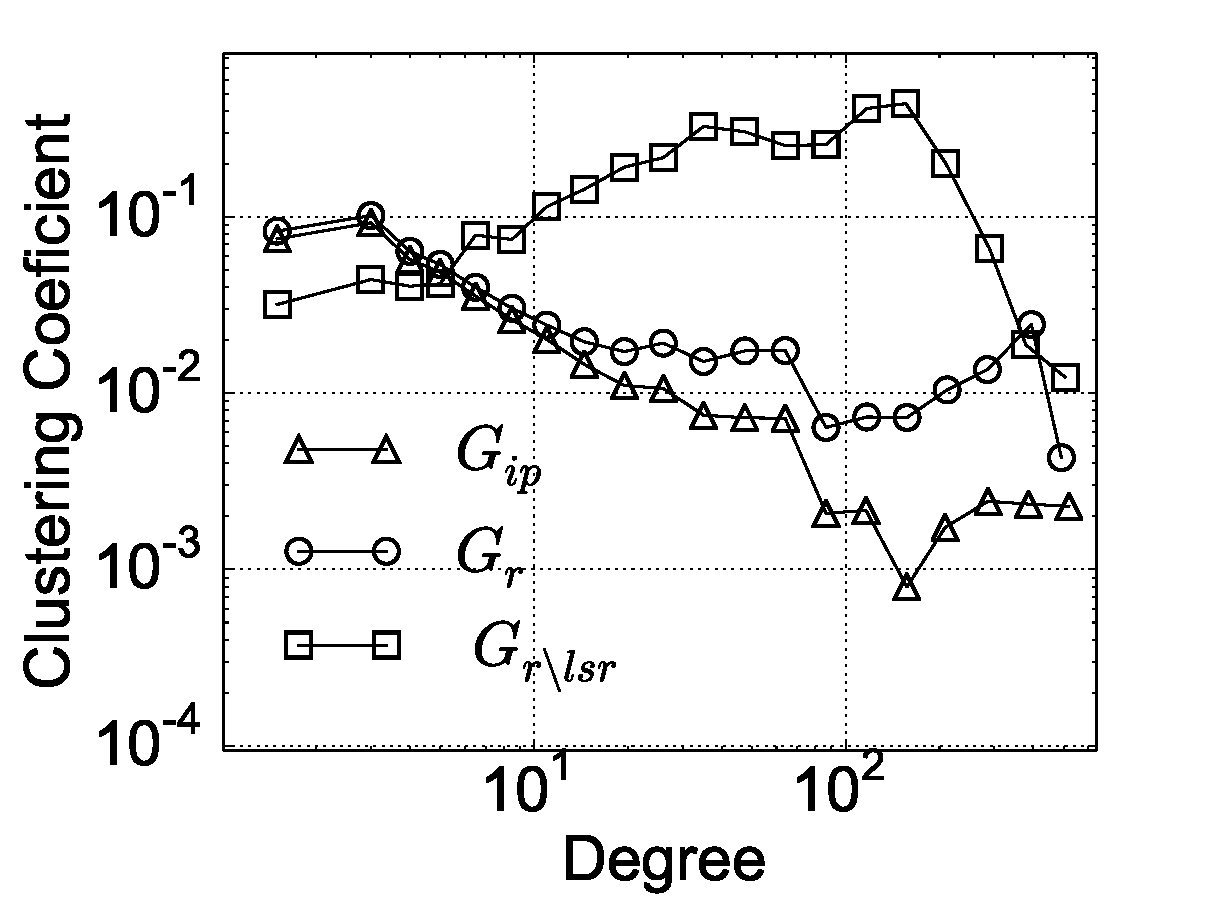
\includegraphics[width=5.5cm]{ClusteringCoeficient}}\hfil
    \subfloat[Neighbor Degree Distribution]{\label{fig_neighbor}
      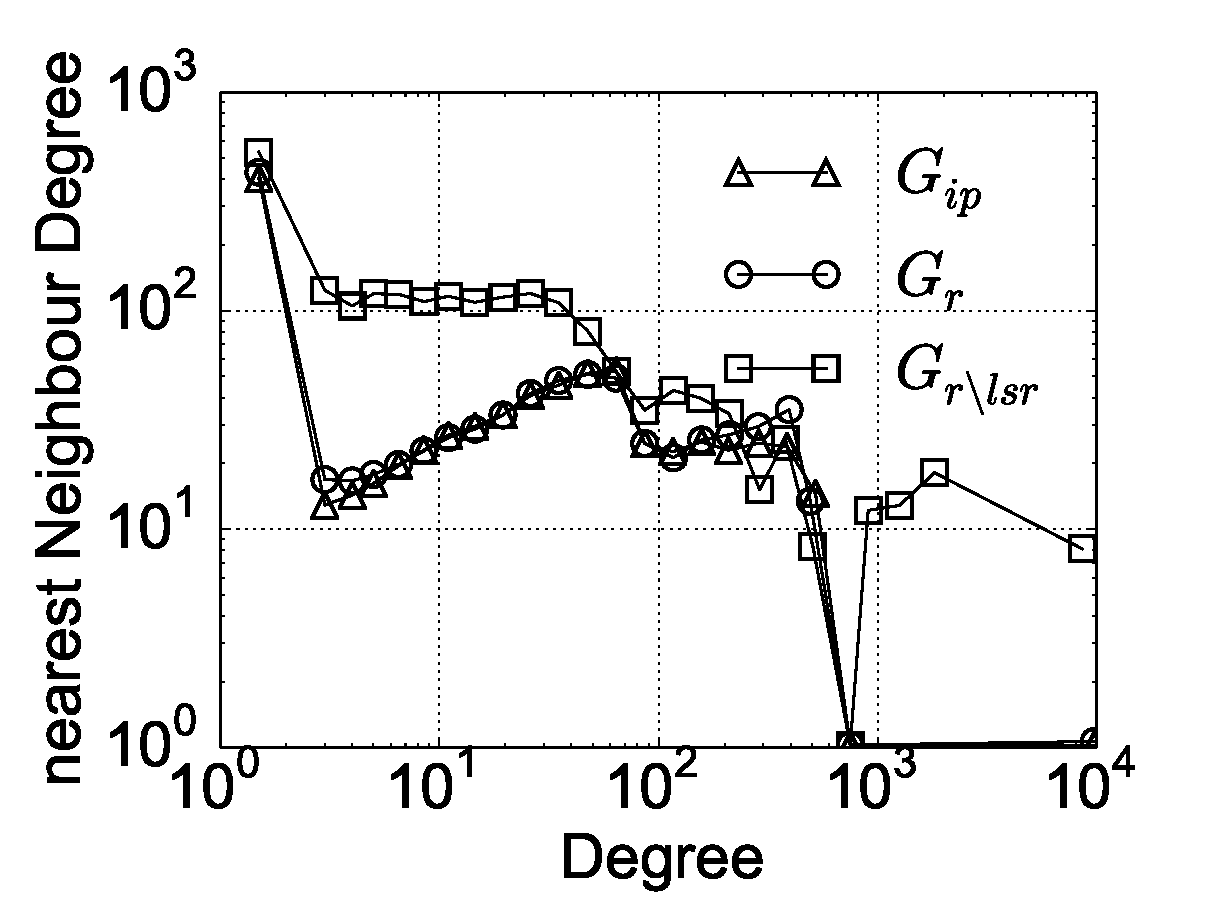
\includegraphics[width=5.5cm]{NearestNeighbor}}
  \end{center}
\caption{\textbf{Metrics for IP, router and MPLS cluster interconnection topologies.} IP, router and MPLS cluster interconnection topologies have similar degree distribution. Clustering Coefficient and Neighbor Degree Distribution do not change significantly between IP level and router level topologies. However the \textit{MPLS clusters} presence highly impact on internet topology. The figure suggest that routers with low degree are highly connected with LSRs (Neighbor Degree Distribution) and routers with high degree usually have \textit{MPLS clusters} as common neighbors (Clustering Coefficient).} \label{fig_metrics}
\end{figure*}

We defined several graphs at different abstraction levels as following: 
%First, we obtained a portion of the IP level topology $G_{ip}$ from traceroutes; noticing that traceroutes reveals just a IP addresses of the incident routers in a path. 
%Secondly, we identified the MPLS tunnels, based on the~\cte{} clasification. 
%Later, we solved the alias resolution process using MIDAR and we develop a router level topology $G_{r}$ (from IP interfaces) and an MPLS router (LSRs) level topology  $G^{mpls}_{r}$ (from IP interfaces belonging to MPLS tunnels). Additionally,  we identified the \textit{MPLS clusters} $C^{mpls}_{i}$ and we treat each cluster as single node in order to study how they interacts with the entire router level topology $G_{r\backslash lsr}$. Finally, in order to better understand the MPLS behaviour  we studied this interaction for some ASes $G_{r\backslash lsr}(as)$.

%Following,  we define with more detail terminology used in this paper. 

\textbf{IP level Graph:} $G_{ip}=(V_{ip}, E_{ip})$, where $V_{ip}$ is the IP address discovered in our exploration and $E_{ip}$ is the set of the links found trough traceroute.
Notice that traceroute just records incident IP addresses in a path.

\textbf{Router Level Graph:} $G_{r}=(V_{r}, E_{r})$, where $V_{r}$ is the set of routers in which at least one IP address using MIDAR, and $E_{r}$ is the set of all the links found between any pair of routers $v\in V_{r}$.

\textbf{MPLS router level Graph:} $G^{mpls}_{r}=(V^{mpls}_{r}, E^{mpls}_{r})$ where  $V^{mpls}_{r}$ is the set of routers in which at least one routers' IP address belongs to an MPLS tunnel, and  $E^{mpls}_{r}$ is the set of all \textit{mpls links} $(v^{mpls}_{r}(i), v^{mpls}_{r}(j))$ such as 
$\{{v^{mpls}_{r}(i)},{v^{mpls}_{r}(j)} \}\in V^{mpls}_{r}$.

\textbf{ASes induced Graphs:} $G_{r}(as)=(V_{r}(as), E_{r}(as))$ and $G^{mpls}_{r}(as)=(V^{mpls}_{r}(as), E^{mpls}_{r}(as))$ are the induced graphs of $G_{r}$ and $G^{mpls}_{r}$ respectively; such that each vertex has a router's interface belonging to the same Autonomous System $as$.

\textbf{MPLS clusters:} $C^{mpls}_{i}$ is a connected component $i$ of $G^{mpls}_{r}(as)$. 
One AS could to have several \textit{MPLS clusters}.    

\textbf{MPLS cluster interconnection Graph:} $G_{r\backslash lsr}=(V_{r\backslash lsr},E^{mpls}_{r\backslash lsr})$ is an hybrid router level graph where all the \textit{MPLS clusters}  $C^{mpls}_{i}$ were contracted to a single node $v\in V_{r\setminus ls}$, and non MPLS capable routers remain unchanged. 
Broadly speaking, an \textit{MPLS cluster interconnection Graph} refers to a router level graph where all \textit{MPLS clusters} are treated as a single node. In this way, we can study how IP interfaces and non MPLS capable routers interact with \textit{MPLS clusters}. 
Additionally, we called $G_{r\backslash lsr}(as)$ to the induced subgraphs of $G_{r\backslash lsr}$ by routers having at least one interface in the Autonomous System $as$.


As the analysis is mainly based on $k$-core decomposition, we present the following definitions:
 
%Formally, let the graph $G=(V,E)$, $k$-core decomposition analysis is defined as:

\begin{itemize}
\item[i]{\textbf{\textit{k}-core:}}. Given a graph $G=(V,E)$, then the subgraph $H=(C,E|C)$ induced by the set $ C\subseteq V$ is a \textit{k}-core of order $k$ $iff$ $\forall v \in C: degree_{H}(v)\geq k$ and $H$ is the maximum subgraph with this property.
%A \textit{k}-core of $G$ can therefore be obtained by recursively removing all the vertices of degree less than $k$, until all vertices in the remaining graph have at least degree $k$. 

\item[ii]\textbf{Shell index}. A vertex $i$ has shell index $c$ if it belongs to the $c$-core but not to $(c+1)$-core. 
We denote by $C_i$ to the shell index of vertex $i$. A shell $C_c$ is composed by all the vertices whose shell index is $c$. The maximum value $c$ such that $C_c$ is not empty is denoted $C_{\max}$. 
Thefore, the $k$-core is thus the union of all shells $C_c$ with $c \geq k$.
\end{itemize}

Finally, we use  \textit{LaNet-vi} \cite{Alvarez06k} to get the $k$-core decomposition. 
This tool returns a two dimensional plot, where the position of each vertex depends on its shell index and on the index of its neighbors. 
A color code allows for the identification of shell indices, while the vertex's original degree is provided by its size, which depends logarithmically on the degree.
A central role in the visualization method is played by multi-components representation of $k$-cores. 
In the most general situation, the recursive removal of vertices having degree less than a given $k$ can break the original network into various connected components, each of which might even be once again broken by the subsequent decomposition.

In this paper, we use $k$-core decomposition focused on properties around \textit{mpls clusters} interconnection. 
 \textit{LaNet-vi} is useful to read basic features of the graph (degree, hierarchical structure, etc.) as well as more entangled features, e.g., the relation between a vertex and the hierarchical position of its neighbors. 
It is also useful to  discriminate between networks with different topological properties and structural arrangement.
This provide us an idea about the structural arrangement and topological properties caused by MPLS usage. 
Additionally,  the visualization help us to find properties and fingerprints tightly related with MPLS presence.


\subsection{MPLS on Internet Topology}\label{cluster.topo}
%%%%%%%%%%%%%%%%%%%%%%%%%%%%%%%%%%%%%%%
%%%%%%%%%%%%%%%%%
\begin{figure*}[!t]
\centering
\subfloat[]{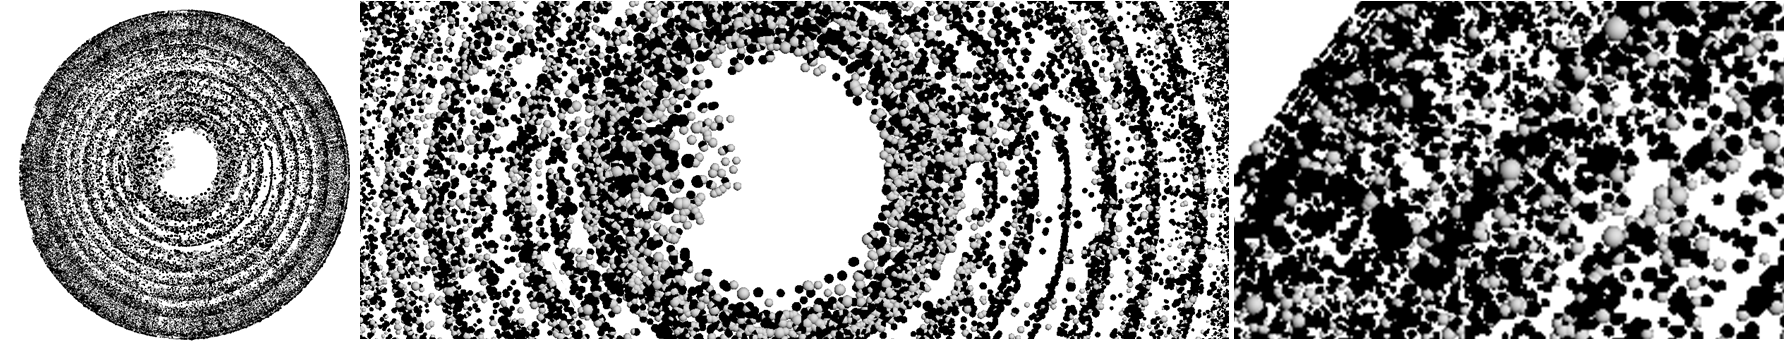
\includegraphics[width=18cm]{LSR}%
\label{fig_k_core_LSR}}
\hfil
\subfloat[]{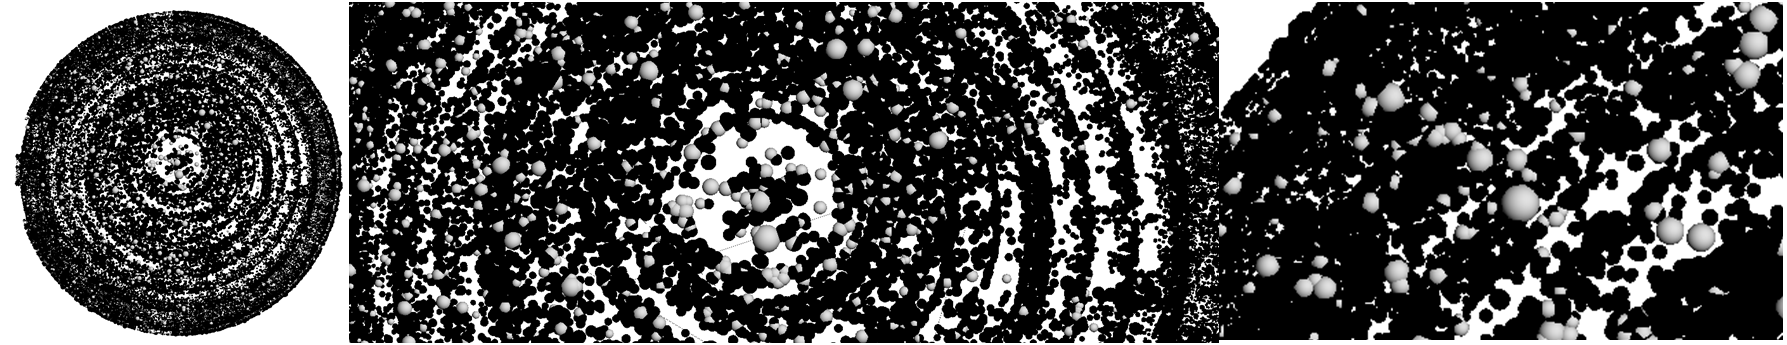
\includegraphics[width=18cm]{MPLS}%
\label{fig_k_core_MPLS}}
\caption{ (a) The $k$-core visualization of router level topology $G_{r}$. Black nodes refer to non MPLS capable routers and gray nodes refer to LSRs. (b) The $k$-core visualization of MPLS cluster level topology  $G_{r\backslash lsr}$. Black nodes refer to non MPLS capable routers and gray nodes refer to \textit{MPLS clusters}.}
\label{fig_kcore_overview}
\end{figure*}

We analyzed the graphs $G_{ip}$ and $G_{r}$ in order to know if there is some strong difference between their structure and properties. 
As was expected we noticed that the router level topology has slightly stronger clustering coefficient than IP level topology (see figure~\ref{fig_clustering}), due to because the join of IP interfaces into single routers. 
However, the main structure of both topologies are similar as it is displayed at figures~\ref{fig_degree_distribution} and~\ref{fig_neighbor}.  
Because we did not notice any meaningful difference between these topologies, and router level topology are more approached to a realistic Internet  one, we use the last one for the remaining of our analysis.

Figure \ref{fig_k_core_routers} shows the $k$-core visualization of $G_{r}$. 
In the center is located the shell index with the $C_{\max}$  and the rest of the shells are located concentrically around it. 
Notice that $C_{\max}$-core is composed by several components with one having the most significant part, and it is shown at left of the center (black nodes).
On the right there is a gray scale with each shell index $c_i$, and on the left it is a node degree scale representing the degree in a logarithmic scale.
We see that all the shells index are highly populated and that the node degree is not related with the shell index, i.e., there are many routers with high degree in the outer (lower) shells. 
Another typical feature of router level topology is that the links between routers mainly occurs between routers belonging to neighbors shells, e.g., the routers on the outer shells are not usually connected to the routers located on the  $C_{\max}$-core, as it is in the Autonomous Systems maps~\cite{Alvarez06k}. 

In order to locate LSRs-routers with MPLS capabilities into the shells index over $k$-core decomposition, we painted in black the \textit{non MPLS capable routers} and in gray color the LSRs. 
The results are showed in figure \ref{fig_k_core_LSR}. 
For the sake of the visualization we do not include neither the shell index, degree scale nor edges between shells. 
We noticed that the LSRs are commonly distributed around the different shells of Internet but  lightly tends to concentrate with more density nearby to the $C_{\max}$-core.
Additionally, we apply the same methodology for the MPLS interconnection cluster level graph $G_{r\backslash lsr}$: \textit{MPLS clusters} (gray nodes) are distinguished from the non MPLS capable routers (black nodes), presented at figure \ref{fig_k_core_MPLS}.
In this case,  \textit{MPLS clusters}  are also spread out on the Internet, indeed we see some well defined gray nodes on the periphery of the decomposition. However \textit{MPLS clusters} shows a stronger tendency to concentrate it near to the $C_{\max}$-core. 

Finally, we evaluated the impact of \textit{MPLS clusters} on the typical router level topology, i.e., \textit{MPLS cluster interconnection graph} $G_{r \backslash lsr }$. We use metrics such as degree distribution, clustering coefficient, and nearest neighbor degree, as is shown on figure \ref{fig_metrics}. 
We noticed that \textit{MPLS clusters} highly impact over the router level topology. 
On one hand, the nearest neighbor degree highly increments for low degrees nodes on $G_{r \backslash lsr }$, suggesting that routers with low degree are highly connected to \textit{MPLS clusters} and thereby to LSRs. 
On the other hand, the clustering coefficient of $G_{r \backslash lsr }$ change significantly their slope in regards with IP and router level topology, indicating that routers with high degree are connected to \textit{common} \textit{MPLS clusters}.


\subsection{\textit{MPLS clusters} on Autonomous Systems}\label{cluster.as}

Although, the previous results give us a general overview about MPLS deployment, we believe that the study of MPLS structure requires some deep into the individual AS topology. 
Indeed, we found that around $89.9\%$ of \textit{mpls links} are intra-AS.  
Thereby, we choose the top of ASes according to the total number of discovered links; and in order to focus our analysis on those ASes were MPLS is relevant, we discarded those having less than five hundred \textit{mpls links}. 
Additionally, we identified  the amount of \textit{mpls links} by AS, distinguishing the type of tunnel: 

\begin{itemize}
\item[i] \textit{explicit mpls link:} Link between an interface $i^{\text{explicitMPLS}}_{n}$  and its previous interface $i^{\text{MPLS}}_{n-1}$ discovered by traceroute, such that $i^{\text{explicitMPLS}}_{n}$ belongs to an explicit MPLS tunnel and $i^{\text{MPLS}}_{n-1}$ belongs to any kind of MPLS tunnel (explicit, \textit{qTTL} based or \textit{u-turn} based).

\item[ii] \textit{qTTL mpls link:} Link between the interfaces $i^{\text{qTTL}}_{n}$  and $i^{\text{MPLS}}_{n-1}$, such that $i^{\text{qTTL}}_{n}$ belongs to a tunnel \textit{qTTL} based.

\item[iii] \textit{u-turn mpls link:} Link between the interfaces $i^{\text{u-turn}}_{n}$  and $i^{\text{MPLS}}_{n-1}$, such that $i^{\text{u-turn}}_{n}$ belongs to a tunnel \textit{u-turn} based.

\end{itemize}

The summary of the top ASes is showed in the figure \ref{top_as}. 
We noticed that the ratio $r_{mpls}= \vert E^{mpls}_{r} (as) \vert /\vert E_{r} (as) \vert $  is greater when more  \textit{explicit mpls links} have been discovered. 
Interestingly, we also see that the ASes with more links discovered have the lowest ratio $r_{mpls}$. 

For our purposes, we select the most representatives ASes from those in figure~\ref{top_as}.
In this way we analyzed the graphs $G_{r}(as)$ and $G_{r\backslash lsr}(as)$ for AS1299, AS174, AS6762, AS7018, AS1273 and AS2914. 
The most remarkable observation (see figure~\ref{fig_cluster_mpls}) occurs regarding the graph $G_{r\backslash lsr}(as)$: $k$-core decomposition highly differs on those ASes, where prevails explicit tunnels in regard to those with more \textit{u-turn} tunnels proportionally. 
We show that \textit{MPLS clusters} (represented as gray nodes) for  AS1299 (Teliasonera AB), AS174 (Congent Communication) and AS6762 (Telecom Italia) are spread out over different shells index. 
These $k$-core structures are similar in our top four of ASes where we additionally noticed  the \textit{u-turn} signature was majority discovered, i.e., between $30\%$ and  $80\%$ over  the total amount of \textit{mpls links}. 
However, for AS7018 (AT\&T), AS1273 (Cable and Wireless Worldwide plc) and AS2914 (NTT America Inc.) %[PAY ATTENTION: THERE IS AS2914 IN YOUR PICTURES, PLEASE FIND IF IT IS 2910 OR 2914 AND CORRECT THEM] GD: Corrected
 where prevail explicit tunnels, we found a $k$-core structure highly different.  
In these cases,  the ASes have few and well defined \textit{MPLS clusters}, mainly belonging to the $C_{\max}$-core. 
The same $k$-core decomposition structure was noticed  on the rest of top ASes with high percentage of \textit{qTTL} signature, i.e., AS7018, AS1273 and AS2914.

Another remarkable observation  relays on the fact that the maximum degree reached by \textit{MPLS clusters} is considerably high in regard to the network size. 
Indeed, with exception of AS174, the rest of ASes suggest that more than $50\%$ of non mpls routers are connected  to at least one LSR. 
Actually, even the outer shells of the $k$-core decomposition are linked directly with the \textit{MPLS clusters} located in the $C_{\max}$-core. 
This behaviour match with our observation of nearest neighbor degree and clustering coefficient noticed on section \ref{cluster.topo}. 
Additionally, because \textit{MPLS clusters} are mainly located on $C_{\max}$-core (even on the ASes with high percentage of \textit{u-turn mpls links}), we believe that MPLS plays an important role in the backbone of the ISPs.

Summarizing, we observed that  $k$-core decomposition structure varies according the type of MPLS tunnels that prevails in the AS. 
This observation could suggest that exists a great number of MPLS links non revealed by traceroute in ye ASes where prevails \textit{u-turn} signatures; therefore, the LSRs discovered can not build large \textit{MPLS clusters} so they are thoroughly spread out. 
Additionally, because \textit{u-turn} signatures are inaccurate, as we showed previously, there could exists several false LSRs spread out over the shell indexes, adding false \textit{MPLS clusters}. 
Finally, it draws our attention that the ratio of \textit{u-turn links} differs greatly just on ASes with low $r_{mpls}$, producing a \textit{u-turn} bias in some ASes while not in others, yielding inaccuracies to topology.


\begin{figure}[!htb]
\centering
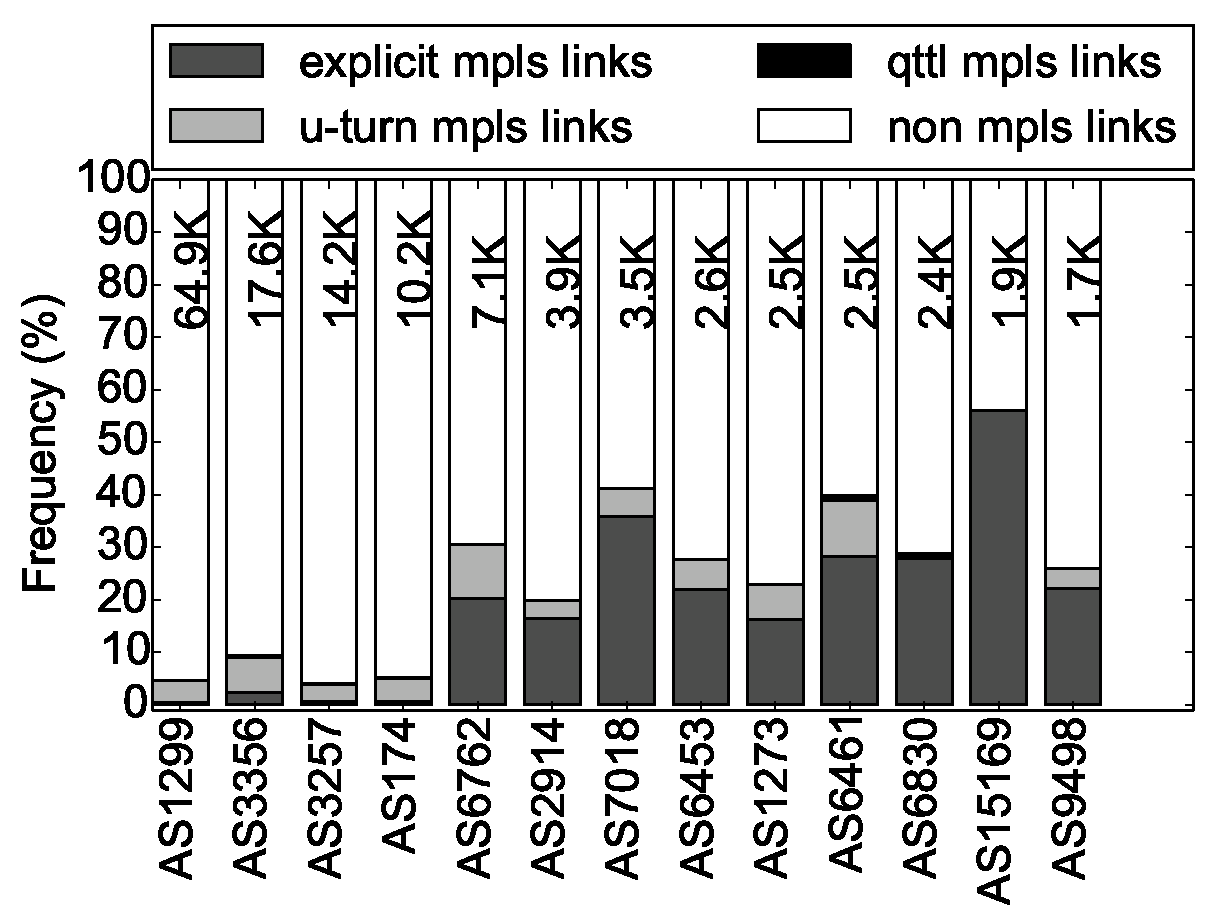
\includegraphics[width=8cm]{TOP_AS}
% where an .eps filename suffix will be assumed under latex, 
% and a .pdf suffix will be assumed for pdflatex; or what has been declared
% via \DeclareGraphicsExtensions.
\caption{\textbf{Top of ASes with most links discovered} On top four ASes prevails \textit{u-turn mpls links}. On the rest of ASes prevails \textit{qttl mpls links}.}
\label{top_as}
\end{figure}

%Figura u-turn
\begin{figure*}[!htb]
\centering
\subfloat[AS1299  Teliasonera AB , $C_{\max}=21$, $\text{Degree}_{\max}=2781$]{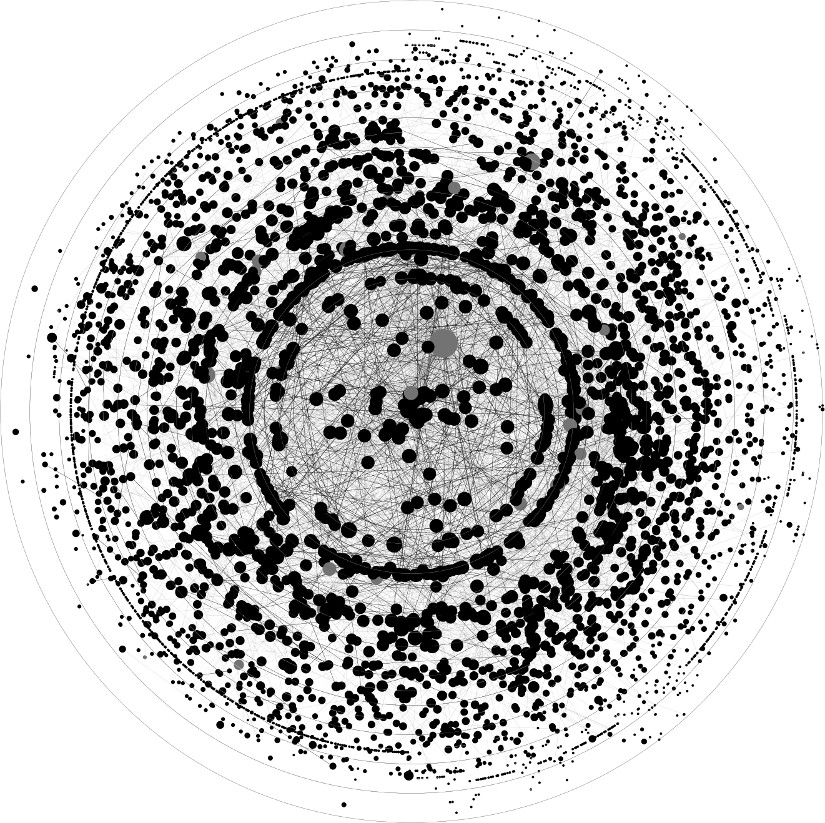
\includegraphics[width=2in]{1299}%
\label{fig_cluster_mpls_1299}}
\hfill
\subfloat[AS174 Congent Communication, $C_{\max}=8$, $\text{Degree}_{\max}=751$]{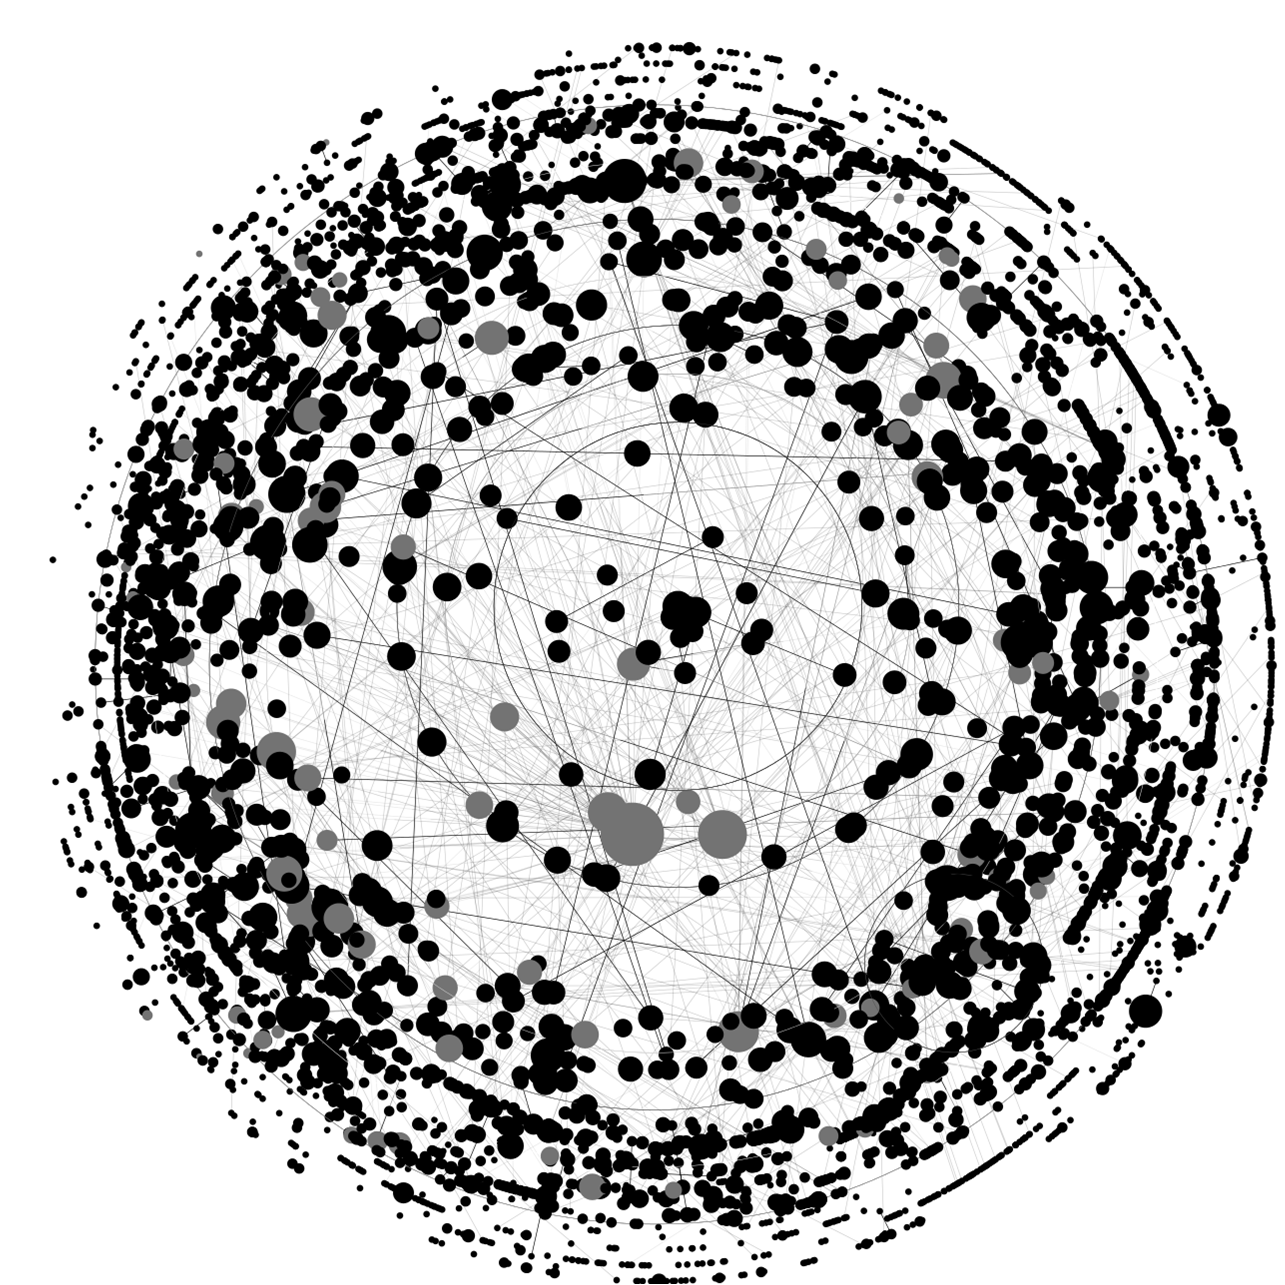
\includegraphics[width=2in]{174}%
\label{fig_cluster_mpls_174}}
\hfill
\subfloat[AS6762 Telecom Italia, $C_{\max}=10$, $\text{Degree}_{\max}=564$]{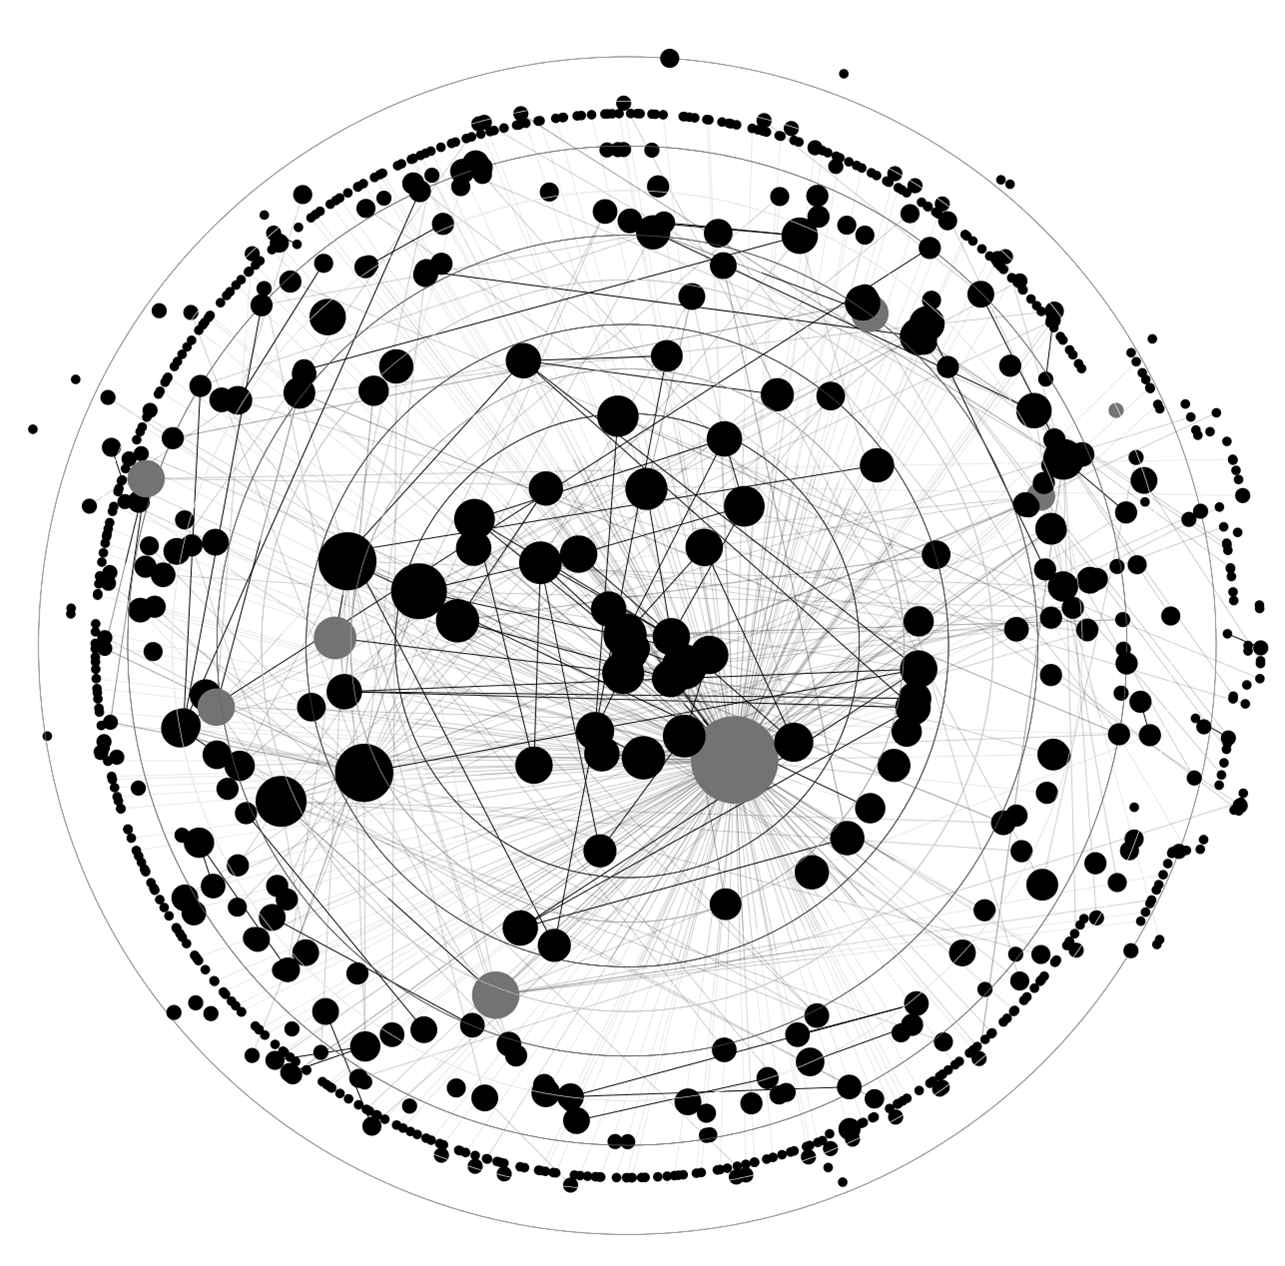
\includegraphics[width=2in]{6762}%
\label{fig_cluster_mpls_6762}}
\hfill
\subfloat[AS7018 AT\&T, $C_{\max}=3$, $\text{Degree}_{\max}=745$]{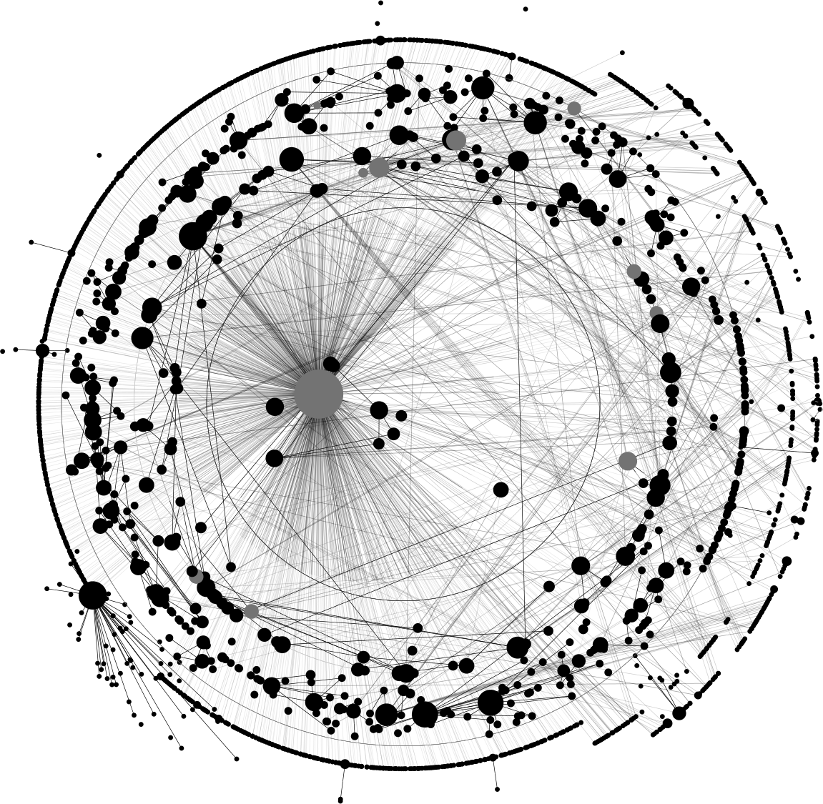
\includegraphics[width=2in]{2914}%
\label{fig_cluster_mpls_2914}}
\hfil
\subfloat[ AS1273 Cable and Wireless Worldwide plc, $C_{\max}=3$, $\text{Degree}_{\max}=806$]{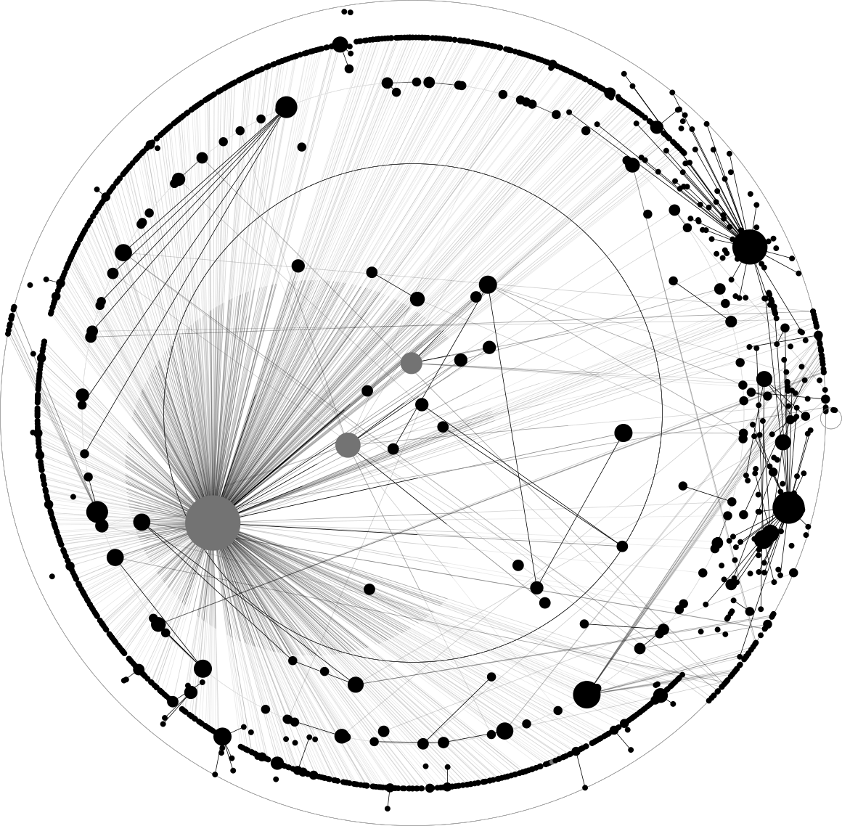
\includegraphics[width=2in]{1273}%
\label{fig_cluster_mpls_1273}}
\hfil
\subfloat[AS2914 Citicorp, $C_{\max}=4$, $\text{Degree}_{\max}=745$]{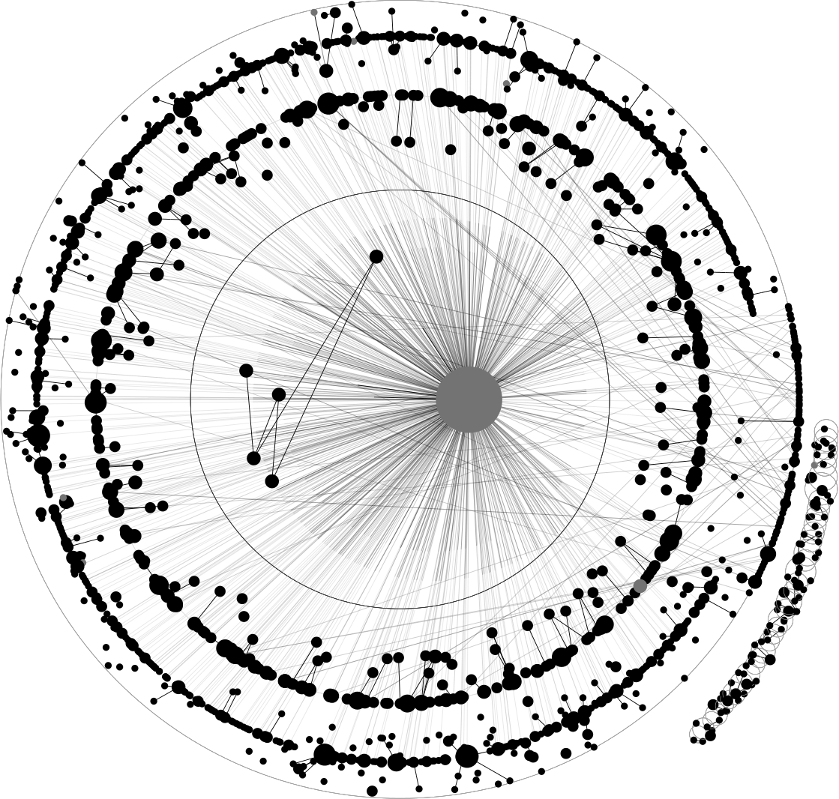
\includegraphics[width=2in]{7018}%
\label{fig_cluster_mpls_7018}}
\caption{\textbf{$k$-core visualization of MPLS cluster interconnection Graph $G_{r\backslash lsr}(as)$}. On the top the ASes show \textit{MPLS clusters} spread out around the shell index of the decomposition. ON the bottom the ASes show \textit{MPLS clusters} well defined and located on the top core $C_{\max}$.}
\label{fig_cluster_mpls}
\end{figure*}